\section{Measurement setup}
\label{sec-testbed}


\textcolor{red}{[Describe the devices we are evaluating]}

In this section, we addressed our testbed in detail. Firstly, we explain our hardware setup, devices' specs, and how they are connected. Knowing hardware testbed, we explain our software environments. Fig \ref{testbed} shows an overview of both hardware and software of our experiments. Eventually, we speak about our performance metrics.

 \subsection{Hardware Testbed}
As Fig. \ref{testbed} exposes, on the left side, we use an off-path \smartnic equipped with a Cortex-72 ARM CPU working at 800 MHz, with 16 cores and 16GB onboard DDR4 memory. It holds a dual-port SFP28 with 25Gbps for each one. It is mounted on the host, which owns an Intel(R) Xeon(R) Silver 4210R CPU working at 2.4GHz, with 10 cores and 32GB memory. Further details regarding cache are reported in Table \ref{cache-size}. Either the host or the \smartnic act as the server machine connecting to a client over a Tofino switch. The client is equipped with an Intel(R) Core(TM) i7-9700 CPU working at 3.0GHz, with 8 cores and 12GB memory. 
\begin{table}[!htb]
\caption{Size of Cache in the host and \smartnic}
\label{cache-size}
\begin{tabular}{|c|c|c|c|c|}
\hline
Device                         & D-Cache & I-Cache & L2   & L3   \\ \hline
\smartnic (ARM) & 512KB   & 768KB   & 8MB  & 12MB \\ \hline
Host (x86)                     & 320KB   & 320KB   & 10MB & 14MB \\ \hline
\end{tabular}
\end{table}


\subsection{Software Setup}
On the server-side, Ubuntu 20.04.1 LTS with kernel 5.4.0-66-generic is installed on the host. The same OS runs on the client machine, as well. Nonetheless, the \smartnic executes Ubuntu 20.0.1 with a modified kernel 5.4.44. 
\par
For implementing our ANNs, we used two frameworks; 
\begin{itemize}
 \item \textbf{TensorFlow}  \cite{abadi2016tensorflow}: We implemented VGG16 \cite{simonyan2014very} with TensorFlow. Our model recognizes type of pets based on the images. We adopted "Cats vs Dogs" dataset \cite{petimages} to train and test our model. Moreover, we compressed the trained model with TensorFlow lite \cite{petimages}, and ran that version on our \smartnic. Note to mention, both machines support floating-point operation, and we do not apply any quantization method.
 \item \textbf{scikit-learn}  \cite{scikit-learn}: By this framework, we implemented the second used case in \cite{siracusano2020running}, with the same dataset, but without any quantization. The neural network is an MLP classifier for anomaly detection in the UNSW-NB15 dataset \cite{UNSW}, having three layers with the size of (32, 16, 2).
\end{itemize}

\begin{figure}[ht!]
\centering
    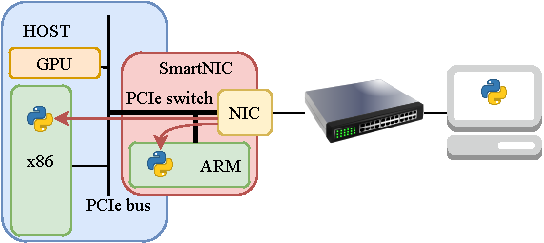
\includegraphics[width=0.47\textwidth]{./figs/testbed.pdf}
    \caption{The testbed}
    \label{testbed}
\end{figure}

\subsection{Workload}
\textcolor{red}{[Describe how we generate the workload in our experiments]}

For evaluating the system, we have developed a socket-based client-server application in Python3. The client program, running on the right-hand machine of Fig. \ref{testbed}, data is read from the dataset; Then, a request is transmitted to the server program, running either on the host or on the \smartnic on the left side Fig. \ref{testbed}, over a TCP connection. The server code runs the model and waits for requests. Once it receives any, it captures and decodes the data, performs the corresponding operations, and finally returns the response to the client. Besides, we can break down the overall latency by adding timestamps in our code. Our implemented codes are released in our Git repository \cite{sdn2021git}

\subsection{Measured resources}
\textcolor{red}{[Describe our metrics and how we measure them in each device]}

Once a neural network is implemented, the first point coming to mind is how accurate it is. With this in mind, in our experiments, we divide our datasets into two parts, training data (80\% of whole data) and test data (the rest 20\% of data). The trained models are evaluated by unseen test data at the end of the training, and the accuracy is measured.
\par
The following parameter reserving some words here is the latency. As we addressed in previous lines, we implemented our code in Python3. We can measure the overall latency in our client program. Once the code sends a request, it also starts the timer. Whenever it captures the response, stops the timer, and calculates the overall latency. With the same timestamping approach, we can break down the latency in the server code to extract communicating time and executing time, as a further illustration. 
\par
To clarify the results, we report roofline results. Roofline, proposed in \cite{10.1007/978-3-319-17248-4_7}, is a benchmark estimating the performance in different levels of caches, memory, and CPU. It reports the maximum bandwidth of caches and memory in terms of GB/s, the maximum computation power of the CPU in terms of GFLPs/sec.
